%-*- coding: UTF-8 -*-
\documentclass[UTF8]{ctexart}
\usepackage{geometry}
\geometry{a4paper,centering,scale=0.8}
\usepackage{graphicx}
\usepackage{amsmath}
\usepackage{textcomp}
\usepackage{amsthm}
\usepackage{amssymb}
\usepackage{float}

\title{\heiti Machine Learning}
\author{卢婧宇}

\begin{document}
\maketitle
\tableofcontents

\newpage
\section{Linear Regression with Multiple Varibles 多变量线性回归}
\subsection{Multiple Features 多维特征}
之前学习的中,关于线性回过问题,只有一个变量,是单变量。现在我们对房价模型增加更多的特征,
例如房间数目、楼层数等等。构成一个含有多个变量的模型,模型中的特征为($x_1,x_2,...,x_n$)。如下图 ~\ref{fig:1} 所示。
\begin{figure}[htb]
 \center{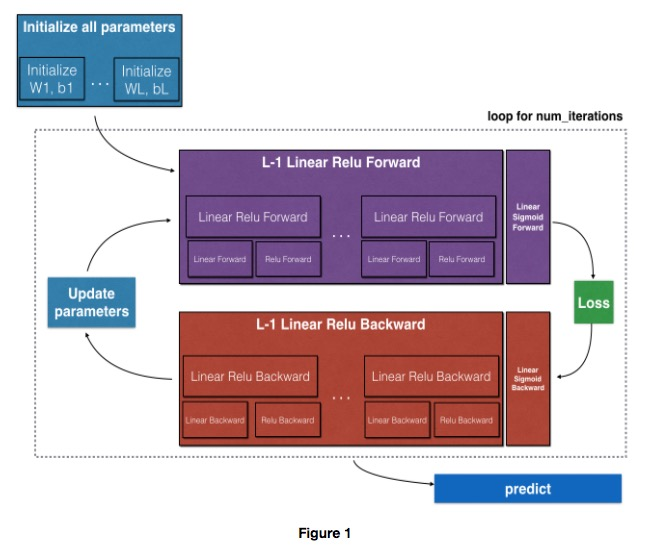
\includegraphics[width=10cm]  {1.jpg}}
 \caption{多特征房屋交易数据}
 \label{fig:1}
 \end{figure}

 Notation:
\begin{itemize}
  \item $n$ = number of features
  \item $x^{(i)}$ = input (features) of $i^{(th)}$ training example.表示第i个样本
  \item $x_j^{(i)}$ = value of feature $j$ in $i^{th}$ training example. 表示第i个样本中第j个特整。
\end{itemize}

有多个变量的Hypotheis:

Previously:

\begin{equation*}
h_\theta(x) = \theta_0 + \theta_1x_1 + \theta_2x_2 + \theta_3x_3 + \theta_4x_4
\end{equation*}

\begin{equation*}
h_\theta(x) = \theta_0 + \theta_1x_1 + \theta_2x_2 + ...+ \theta_nx_n
\end{equation*}

For convenience of notation,define $x_0$=1.

用向量表示:

\begin{equation*}
  x=
  \begin{bmatrix}
    x_0\\
    x_1\\
    x_2\\
    ...\\
    x_n
  \end{bmatrix} \qquad
  \theta^{T} =
   \begin{bmatrix}
     \theta_0 & \theta_1 & \theta_2 & ... & \theta_n
   \end{bmatrix}
\end{equation*}

\begin{equation*}
  h_\theta(x) = \theta_0 + \theta_1x_1 + \theta_2x_2 + ...+ \theta_nx_n
  =\theta^{T}x
\end{equation*}

\subsection{Graadient Descent for Multiple Varibles 多变量梯度下降}
之前提到的一种线性回归的假设形式,这是一种有多特征或者多变量的形式。在本节中将找到满足这一假设的参数,用梯度下降法解决多特征的线性回归问题。

Hypothesis:
\begin{equation*}
  h_\theta(x) =\theta^{T}x = \theta_0 + \theta_1x_1 + \theta_2x_2 + ...+ \theta_nx_n
\end{equation*}

Parameters:
\begin{equation*}
  \theta_0,\theta_1,...,\theta_n
\end{equation*}

不要把$\theta_n$想成是n+1个单独的参数,把这n+1个$\theta$参数想象成一个n+1维的向量$\theta$。

Cost function:
\begin{equation*}
  J(\theta_0,\theta_1,...,\theta_n)=
  \frac{1}{2m}
  \sum^m_{\substack{i=1}}
   \Big(h_\theta(x^{(i)})-y^{(i)}\Big)^{2}
    = \frac{1}{2m}
   \sum^m_{\substack{i=1}}
    \Big((\sum^n_{\substack{j=0}}
    \theta_jx_j^{(i)})-y^{(i)}\Big)^{2}
\end{equation*}

同样不要把函数J想成是一个关于n+1个自变量的函数,而是看成带有一个n+1维向量的函数。

Gradient descent:
\begin{equation*}
Repeat:
  \theta_j := \theta_j - \alpha
  \frac{\partial}{\partial\theta_j}
  J(\theta_0,...,\theta_n)=\theta_j - \alpha
  \frac{\partial}{\partial\theta_j}J(\theta)
\end{equation*}

simultaneously update for every j=0,...,n

Gradient Descent:

Previously(n=1),Repeat:
\begin{equation*}
  \theta_0 := \theta_0 - \alpha
  \frac{1}{m}
  \sum^m_{\substack{i=1}}
   \Big(h_\theta(x^{(i)})-y^{(i)}\Big)
\end{equation*}
\begin{equation*}
  \theta_1 := \theta_1 - \alpha
  \frac{1}{m}
  \sum^m_{\substack{i=1}}
   \Big(h_\theta(x^{(i)})-y^{(i)}\Big)x^{(i)}
\end{equation*}

simultaneously update $\theta_0,\theta_1$

New algorithm(n>1),Repeat:
\begin{equation*}
  \theta_j := \theta_j - \alpha
  \frac{1}{m}
  \sum^m_{\substack{i=1}}
   \Big(h_\theta(x^{(i)})-y^{(i)}\Big)x_j^{(i)}
\end{equation*}

simultaneously update $\theta_j$ for j=0,...,n

其实多参数和两个参数的形式一样只不过$x$的下标有变化,对于$\theta_0$,$x_0^{(i)}=1$。
\subsection{Gradient descent in pratice 1:Feature Scaling 梯度下降法实践1-特征缩放}
本节课是关于梯度下降运算中的实用技巧,以及一种方法叫特征缩放(feature scaling)。在面对多维特征问题时,我们要保证这些特征都具有相同的尺度,
这将帮助下降算法更快的收敛。

以房价问题为例,有两个特征,房屋的尺寸和房间的数量,尺寸的值为0-2000平方英尺,而房间数量的值是0-5,
以两个参数分别为横纵坐标,绘制代价函数的等高线图,可以看出图像很扁,梯度下降算法需要非常多次的迭代才能收敛。
解决方法是尝试将所有特征的尺度都尽量缩放到-1到1之间。如图 ~\ref{fig:2} 所示。
\newline


\begin{figure}[htb]
 \center{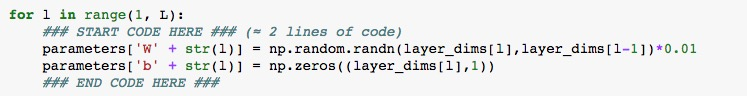
\includegraphics[width=12cm]  {2.jpg}}
 \caption{等高线图}
 \label{fig:2}
 \end{figure}
从上图可以看出有效的方法就是进行特征缩放,这使得等高线图变得圆一些,得到的梯度下降算法可以更快的收敛。
更一般的,我们执行特征缩放时,将特征的取值约束到-1到+1的范围内。这个范围在这附近都可以只要不差太大(大太多或者小太多)。

Mean normalization:

Replace $x_i$ with $x_i-\mu_i$ to maje features have approximately zero mean(Do not apply to $x_0=1$).

就是用特征减去平均值,再除以范围,来替换原来的特征,范围的意思是最大值减最小值。
不管怎样这些取值都是非常近似的,只要将特征转换为相近的范围就都是可以的。特征缩放其实并不需要太精确,只是为了让梯度下降能够更快一点,循环次数少。
\subsection{Gradient descent in pratice 2:Lreaning Rate 梯度下降法实践2-学习率}
本小结将围绕学习率$\alpha$展开,这是梯度下降算法的更新规则(Debugging),也就是如何确定梯度下降是正常工作的,并且如何选择$\alpha$。
如图 ~\ref{fig:3} 所示。
\begin{figure}[htb]
 \center{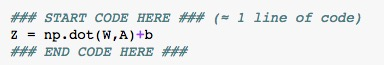
\includegraphics[width=9cm]  {3.jpg}}
 \caption{迭代结果}
 \label{fig:3}
 \end{figure}

从图中可以看出横轴代表迭代次数(No.of iterations),纵轴代表每次迭代后得到$\theta$得到$J(\theta)$的值。

 另外,也可以进行一些自动收敛测试,也就是用一种算法测试梯度下降算法是否已经收敛。如果代价函数$J(\theta)$的下降小于一个很小
的值$\varepsilon$,那么就认为已经收敛,比如可以选择$10^{-3}$,但通常要选择一个合适的阈值$\varepsilon$是相当困难的。所以通常是观察曲线图。

梯度下降算法的每次迭代受到学习率的影响,如果学习率$\alpha$过小,则达到收敛所需要的迭代次数会非常高;
如果学习率$\alpha$过大,每次迭代可能不会减小代价函数,可能会越过局部最小值导致无法收敛。

通常可以考虑尝试的一些学习率:$\alpha$=0.01,0.03,0.1,0.3,1,3,10

\subsection{Features and polynomial regrssion 特征和多项式回归}
多项式回归可以使得用线性回归的方法来拟合非常复杂的函数,甚至是非线性函数。以预测房价为例如图 ~\ref{fig:4} 所示。
\begin{figure}[htb]
 \center{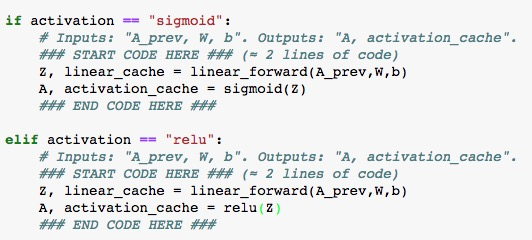
\includegraphics[width=10cm]  {4.jpg}}
 \caption{房屋图形}
 \label{fig:4}
 \end{figure}

假设有两个特征,临街宽度和房屋深度:

\begin{equation*}
h_\theta(x)=\theta_0+\theta_1 \times frontage+\theta_2 \times depth
\end{equation*}

$x_1$=frontage(临街宽度),$x_2$=depth(纵向深度),$x$=frontage$\ast$depth=area(面积),得到:

\begin{equation*}
h_\theta(x)=\theta_0+\theta_1x
\end{equation*}

通过定义新的特征,确实会得到一个更好的模型,与选择的想法密切相关的一个概念被称为多项式回归(polynaoial regression)。
线性回归并不适用于所有数据,有时候我们需要用二次模型去拟合数据:

\begin{equation*}
h_\theta(x)=\theta_0+\theta_1x_1+\theta_2x_2^{2}
\end{equation*}

或者三次方模型:

\begin{equation*}
h_\theta(x)=\theta_0+\theta_1x_1+\theta_2x_2^{2}+\theta_3x_3^{3}
\end{equation*}

如图 ~\ref{fig:5} 所示,为房价的数据,我们需要选择合适的模型拟合数据。
\begin{figure}[htb]
 \center{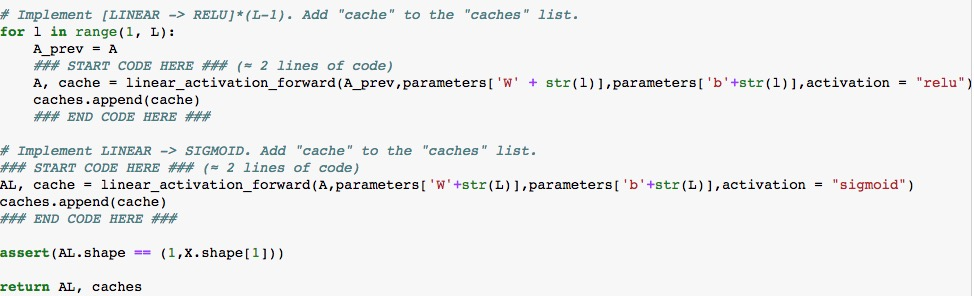
\includegraphics[width=11cm]  {5.jpg}}
 \caption{房屋数据}
 \label{fig:5}
 \end{figure}

通常需要先观察数据再决定准备尝试怎样的模型:
\begin{eqnarray*}
  h_\theta(x) & = & \theta_0+\theta_1x_1+\theta_2x_2+\theta_3x_3 \\
  & = & \theta_0+\theta_1(size)+\theta_2(size)^{2}+\theta_3(size)^{3}
\end{eqnarray*}

其中:$x_1=(size), x_2=(size)^{2},x_3=(size)^{3}$。

除了三次方模型还有其他模型:
\begin{equation*}
h_\theta(x)=\theta_0+\theta_1(size)+\theta_2\sqrt{(size)}
\end{equation*}

注意一点非常重要!如果我们采用多项式回归模型,在运行梯度下降算法前,特征缩放非常有必要,将缩放后的值带入再计算。

\subsection{Normal Equation 正规方程}
对于某些线性回归问题,用正规方程法求解参数$\theta$的最优值更好,与其使用迭代算法,可以一次性求解$\theta$的最优值。
如:

Intuition: If 1D ( $\theta \in \mathbb{R} $)
\begin{equation*}
J(\theta)=a\theta^{2}+b\theta+c
\end{equation*}

正规方程是通过求解下面的方程来找出使得代价函数最小的参数的:
\begin{equation*}
 \frac{\partial}{\partial\theta_j}
 J(\theta_j)=0
\end{equation*}

假设训练集特征矩阵为X(包含了$X_0$)并且训练集结果为向量y,则利用正规方程解出向量:
\begin{equation*}
  \theta=(X^{T}X)^{-1}X^{T}y
\end{equation*}
上标T代表矩阵转置,上标-1代表矩阵的逆。设矩阵A=$X^{T}X$,则:$(X^{T}X)^{-1}=A^{-1}$

以下表示数据为例,如图 ~\ref{fig:6}所示:

\begin{figure}[htb]
 \center{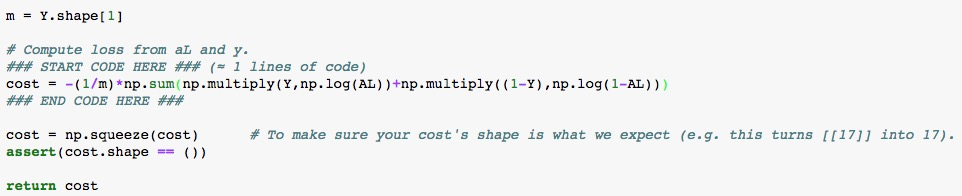
\includegraphics[width=11cm]  {6.jpg}}
 \caption{数据列表}
 \label{fig:6}
 \end{figure}

在Octave中,正规方程写作:
\begin{equation*}
 pinv(X^{'}*X)*X^{'}*y
\end{equation*}
不可逆矩阵正规方程方法不可用。

梯度下降法与正规方程方法的比较:
\begin{itemize}
 \item 梯度下降需要选择学习率$\alpha$,正规方程不需要。
 \item 梯度下降需要多次迭代,正规方程一次运算得出。
 \item 梯度下降当特征数量n大时也能较好适用,正规方程需要计算$(X^{T}X)^{-1}$,如果特征数量n较大则运算代价大,
 因为矩阵逆的计算时间复杂度为O($n^{3}$),通常来说当n小于10000时还是可以接受的。
 \item 梯度下降适用于各种类型的模型,正规方程只适用于线性模型,不适合逻辑回归模型等其他模型。
\end{itemize}

 总结一下,只要特征变量的数目并不大,标准方程是一个很好的计算参数$\theta$的替代方法。
 具体地说,只要特征变量数量小于一万,我通常使用标准方程法,而不使用梯度下降法。

 对于那些更复杂的学习算法,
我们将不得不仍然使用梯度下降法。因此,梯度下降法是一个非常有用的算法,可以用在有大量特征变量的线性回归问题。

\subsection{Normal Equation Noninvertibility(Optional) 正规方程及不可逆性}
当计算$\theta=(X^{T}X)^{-1}X^{T}y$=$inv(X^{'}X)X^{'}y$,那些对于矩阵$X^{-1}X$的结果是不可逆的情况该怎么办?

在数学中我们称不可逆的矩阵为奇异矩阵或退化矩阵。问题的重点在于$X^{'}X$不可逆的问题很少发生。在Octave里,如果你用它来实现$\theta$
的计算,你将会得到一个正常的解。在Octave里,有两个函数可以求解矩阵的逆,一个被称为pinv(),另一个是inv(),这两者之间的差异是些许计算过程上的,一个是所谓的伪逆,但算法执行的流程是正确的,
另一个被称为逆。使用pinv()函数可以展现数学上的过程,即便矩阵X\'X是不可逆的。在pinv()和inv()之间,又有哪些具体区别?

What if $X^{T}X$ is non-invertible?
\begin{itemize}
  \item Redundant features (linearly dependent).

        E.g. $x_1$ = size in $feet^{2}$

             $x_2$ = size in $m^{2}$
  \item Too many features(e.g. m $\leq$ n).

        \- Delete some features,or use regularization.
\end{itemize}

Solutions to the above problems include deleting a feature that is linearly dependent
with another or deleting one or more features when there are too many features.

inv()引入了先进的数值计算的概念。例如,在预测住房价格时,如果$x_1$是以英尺为尺寸计算的房子,$x_2$
是以平方米为尺寸规格计算的。1米等于3.28英尺(四舍五入到两位小数),这样两个特征值满足约束:$x_1=x_2\ast(3.28)^{2}$。

实际上,你可以用这样的一个线性方程,来展示那两个相关联的特征值,矩阵$X^{'}X$将是不可逆的。

第二个原因是有大量的特征值时间学习算法,可能会导致矩阵$X^{'}X$的结果是不可逆的。例如,当m$\leq$n时,m等于10个训练样本n等于100个特征数量。
要找到合适的(n+1)维参数矢量$\theta$这是第 n+1维。尝试从10个训练样本中找到满足101个参数的值,工作量巨大。

如何使用小数据样本以得到100或101个参数,通常使用一种叫做正则化的线性代数方法,通过删除某些特征或是使用某些技术,来解决当m比n小
的时候的问题。即使你有一个相对较小的训练集,也可以使用很多的特征来找到很多合适的参数。

总之,当发现矩阵$X^{'}X$的结果是奇异矩阵,或者找到的其它矩阵是不可逆的。

首先,看特征值里是否有一些多余的特征,像$x_1x_2$是线性相关的,互为线性函数。同时,当有一些多余的特征是,可以删除这两个重复特征里的其中一个,无需两个特征
同时保留,将解决不可逆问题。如果特征数量实在太多删除些用较少的特征来反映尽可能多内容,否则我会考虑使用正规化方法。

\section{Octave Tutorial Octave 教程}

Working on and submitting programming exercises.
\subsection{Basic Operation 基本操作}

可以做基本的算术运算。逻辑运算:$\=\=$ 、$\~\=$ 不等于、$\&\&$ 与、$or$ 或、$xor$ 异或。在终端执行Octave时左边会有
其版本的提示,如果不想看到那个提示,隐藏命名为:PS1('>> '); 但MATLAB中没有。

谈到变量。如果想分配一个a赋值为3,并按下回车键,显示变量a等于3。如果你想分配一个变量但不希望屏幕上显示结果,在命令后加分号。
如图~\ref{fig:7}所示
\begin{figure}[htb]
 \center{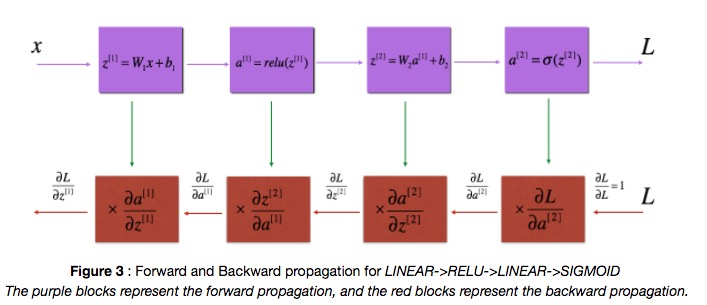
\includegraphics[width=11cm]  {7.jpg}}
 \caption{变量赋值}
 \label{fig:7}
 \end{figure}

如果你想打印出变量,或显示一个变量输入变量名,或者只要输出值用disp(变量名),对于更复杂的屏幕输出也可以用DISP命令显示。也可以用该命令
来显示字符串输入disp sprintf 。如图~\ref{fig:8}所示。
\begin{figure}[H]
 \center{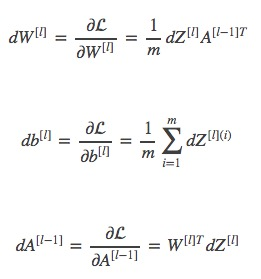
\includegraphics[width=8cm]  {8.jpg}}
 \caption{变量打印}
 \label{fig:8}
 \end{figure}

这是一种,就风格的C语言语法。也有一些控制输出长短格式的快捷键命令,如图~\ref{fig:9}所示
\begin{figure}[H]
 \center{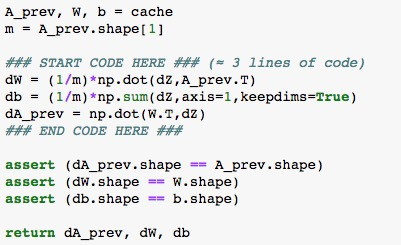
\includegraphics[width=8cm]  {9.jpg}}
 \caption{变量打印}
 \label{fig:9}
 \end{figure}

向量和矩阵。建立一个矩阵A,对矩阵A进行赋值,建立行向量列向量。如图~\ref{fig:10}所示。
\begin{figure}[H]
 \center{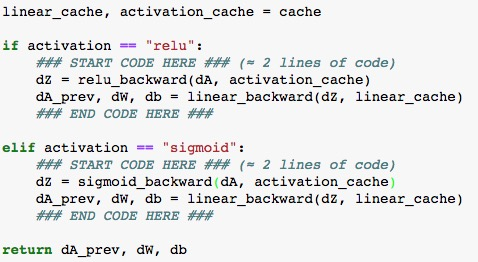
\includegraphics[width=8cm]  {10.jpg}}
 \caption{向量和矩阵}
 \label{fig:10}
 \end{figure}

下面是一些更为有用的符号,如 V=1:0.1:2。V是一组值,从数值1开始,增量或说步长为0.1,直到增加到2,按照这样的方法对向量V操作,可以得到一个行向量,
这是一个1行11列的矩阵的矩阵,其矩阵的元素是1 1.1 1.2 1.3 以此类推,直到2。也可以建立一个集合V并用命令``1:6''进行赋值,这样V就被赋值了1至6的六个整数。
如图~\ref{fig:11}所示。
\begin{figure}[H]
 \center{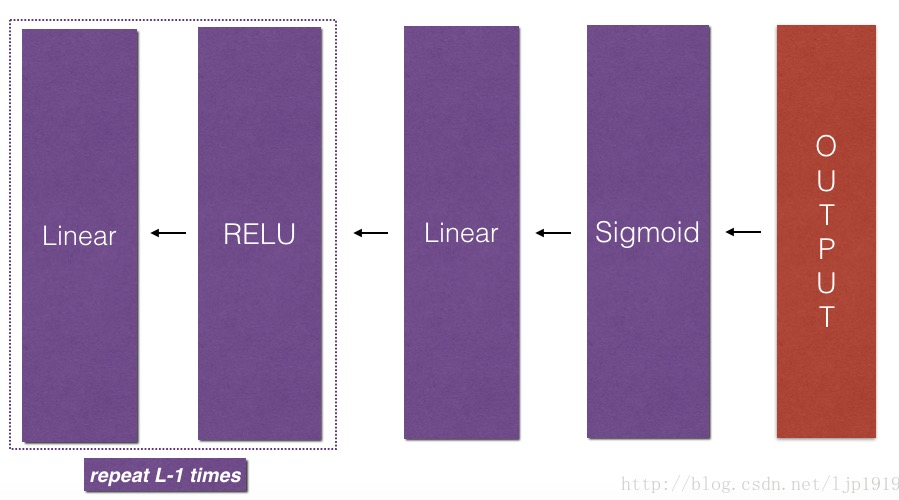
\includegraphics[width=11cm]  {11.jpg}}
 \caption{向量和矩阵}
 \label{fig:11}
 \end{figure}

还有一些生成矩阵的方法。如图~\ref{fig:12}所示
如图~\ref{fig:12}所示。
\begin{figure}[H]
 \center{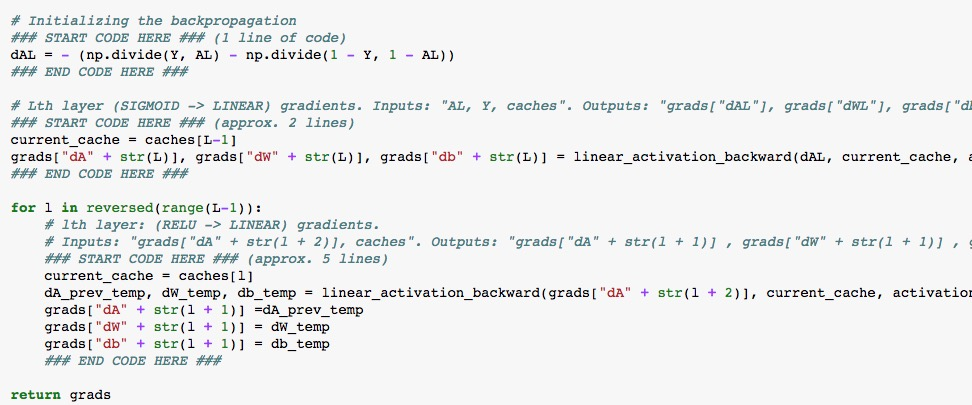
\includegraphics[width=7cm]  {12.jpg}}
 \caption{向量和矩阵}
 \label{fig:12}
 \end{figure}

用rand命令建立一个一行三列的矩阵,元素均为随机值:rand(1,3)。数值介于0和1之间,我们可以得到数值均匀介于0和1之间的元素。

如果知道什么是高斯随机变量什么是正态分布的随机变量。标准正态分布期望值为0,标准差为1。randn是均值为0方差为1的正态分布。randn(n)或rand(n)生成n$\ast$n的随机数矩阵。
rand(n,m)或randn(m,n)生成m*n的随机数矩阵。

产生一个随机分布的指定均值和方差的矩阵:将randn产生的结果乘以标准差,然后加上期望均值即可。并用hist命令绘制直方图。如图~\ref{fig:13}所示
\begin{figure}[H]
 \center{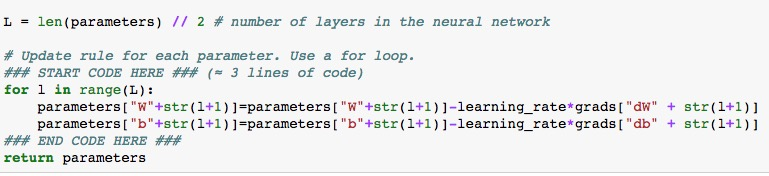
\includegraphics[width=9cm]  {13.jpg}}
 \caption{向量和矩阵}
 \label{fig:13}
 \end{figure}

绘制单位矩阵:I=eye(6)

如果对命令不清楚,建议用help命令:help eye 、help rand 、help help。

\subsection{Moving Data Around 移动数据}
size()命令返回矩阵的尺寸。输出的是一行两列的矩阵,第一个元素是所求矩阵的行数,第二个元素的所求矩阵的列数。可以用sz来存放。
输入size(sz)看看sz的尺寸,返回1 2。

输入size(A,1),将返回3,这个命令会返回A矩阵的第一个维度的尺寸,也就是A矩阵的行数。
同样,命令size(A,2),将返回2,也就是A矩阵的列数。

如果你有一个向量v,假如v=[1 2 3 4],然后输入length(v),这个命令将返回最大维度的大小,返回4。
通常还对向量使用length命令,而不是对矩阵使用length命令,比如length([1;2;3;4;5]),返回5。

当打开Octave时,我们通常已经在一个默认路径中,这个路径是Octave的安装位置,pwd命令可以显示出Octave当前所处路径。
cd 命令,意思是改变路径: cd ` \~ \/ Desktop'。ls查看路径下文件。

如何将文件中的数据读入Octave。只需要键入 featuresX.dat(load features),这样就加载了featuresX文件。同样可以加载 priceY.dat。
其实有好多种办法可以完成,如果你把命令写成了一个字符串的形式:load(`featureX.dat'),也是可以的,只不过把文件名写成了一个
字符串的形式,现在文件名被存在一个字符串中。Octave中使用引号来表示字符串。

另外who命令,能显示出在我的Octave工作空间中的所有变量。同样还有一个whos命令,能更详细地进行查看。

如果你想删除某个变量,你可以使用clear命令,我们键入 clear featuresX,然后再输入 whos 命令,featuresX消失了。

如何存储数据? v=princeY(1:10) 表示将向量Y的前10个元素存入v中。假如我们想把它存入硬盘,那么用 save hello.mat v 命令,这个命令
会将变量v存成一个叫 hello.mat的文件,回车后桌面就出现了一个新文件,名为 hello.mat。

直接键入clear,这样将删除工作空间中的所有变量,所以现在工作空间中啥都没了。

但如果载入hello.mat文件,又重新读取了变量v,因为我之前把变量v存入了hello.mat文件中,所以save命令就是把数据按照二进制形式存储,
或者说更压缩的二进制形式,因此,如果v是很大的数据,那么压缩幅度也很大,占用空间也更小。如果你想把数据存成一个人能看懂的形式,
那么可以键入:

save hello.txt v \-ascii

这样就会把数据存成一个文本文档,或者将数据的ascii码存成文本文档。桌面会有hello.txt文件。如果打开它,我们可以发现这个文本文档存放着我们的数据。
这就是读取和存储数据的方法。

操作数据的方法:假设A还是之前的矩阵。键入A(3,2),将索引第三行第二列的元素。也可以键入A(2,:)来返回A矩阵第二行的所有元素,A(:,2)来返回
A矩阵第二列的所有元素。如图~\ref{fig:14}所示。
\begin{figure}[H]
 \center{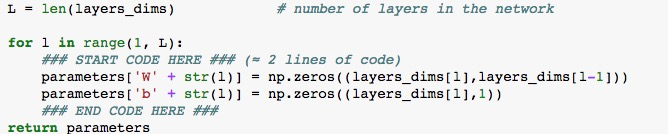
\includegraphics[width=10cm]  {14.jpg}}
 \caption{向量和矩阵}
 \label{fig:14}
 \end{figure}

你也可以在运算中使用这些较为复杂的索引。A([1 3],:),这个命令的意思是取A矩阵的第一行和第三行的每一列,冒号表示的是取这两行的每一列元素。
A(:,2)=[10;11;12],把A的第二列元素重新赋值。A=[A,[100;101;102]],重新添加一列。如图~\ref{fig:15}所示。
\begin{figure}[H]
 \center{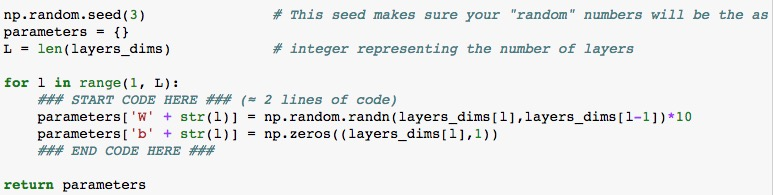
\includegraphics[width=9cm]  {15.jpg}}
 \caption{向量和矩阵}
 \label{fig:15}
 \end{figure}

最后还有一个小技巧,如果你就输入A(:),这是一个特别的语法结构,意思是把A中的所有元素放入一个单独的列向量,这样我们就得到了一个9$\times$1
的向量,这些元素都是A中的元素排列起来的。

矩阵的合并,如图~\ref{fig:16}所示。
\begin{figure}[H]
 \center{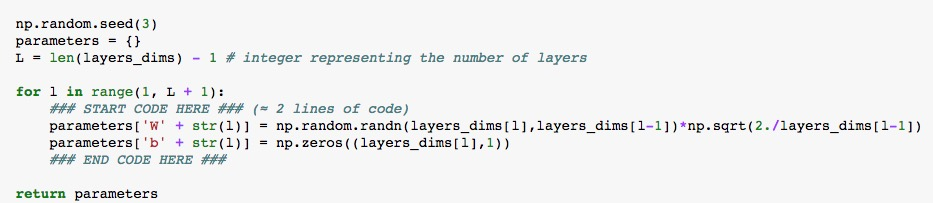
\includegraphics[width=5cm]  {16.jpg}}
 \caption{矩阵合并}
 \label{fig:16}
\end{figure}

还可以C=[A;B]将A和B矩阵上下放在一起。

\subsection{Computing on Data 计算数据}
首先初始化一些变量,设置A为一个3$\times$2的矩阵,设置B为一个3$\times$2矩阵,设置C为2$\times$2矩阵。

计算两个矩阵的乘积。键入A$\times$C,得到一个3$\times$2矩阵。

对每个元素做运算。方法是做点乘运算 A.\* B,将A中的每一个元素与矩阵B中的对应元素相乘,就是两个矩阵元素位运算。
Octave中点号一般用来便是元素位运算。如图~\ref{fig:17}所示。输入A.\^{}2将对每个元素做平方。
\begin{figure}[H]
 \center{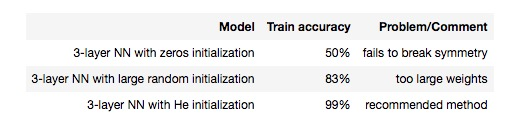
\includegraphics[width=5cm]  {17.jpg}}
 \caption{矩阵元素位运算}
 \label{fig:17}
\end{figure}

设一个列向量V=[1;2;3],键入1.$/$V,得到每一个元素的倒数,所以会分别算出 $1/1、1/2、1/3$。
矩阵也可以这样操作,1.$/$A得到A中每一个元素的倒数。如图~\ref{fig:18}所示。
\begin{figure}[H]
 \center{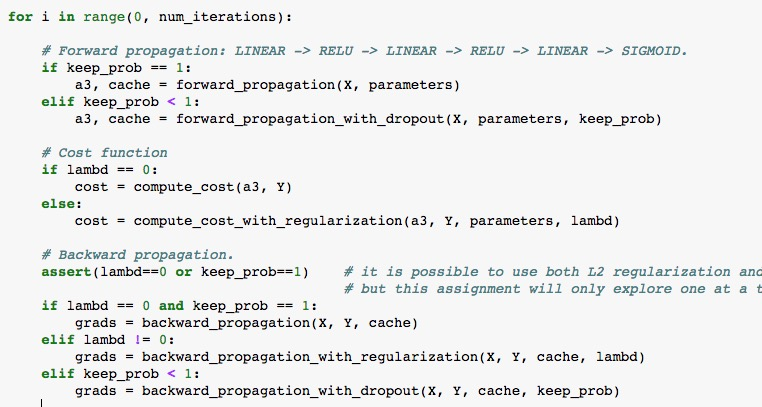
\includegraphics[width=5cm]  {18.jpg}}
 \caption{求倒数}
 \label{fig:18}
\end{figure}

对数运算,对每个元素进行求对数运算log(V)。还有自然数e的幂次运算,以e为底,这些元素为幂的运算exp(V)。
用abs来对V的每一个元素求绝对值abs(V)。$-V$等价于$-1$乘以V,一般就直接用$-V$。

对每个元素都加1。首先构造一个3行1列的1向量,然后把这个1向量跟原来的向量相加。用length(V)命令,ones(length(V),1)
就相当于ones(3,1)。另一种更简单的方法直接用$V+1$。如图~\ref{fig:19}所示。
\begin{figure}[H]
 \center{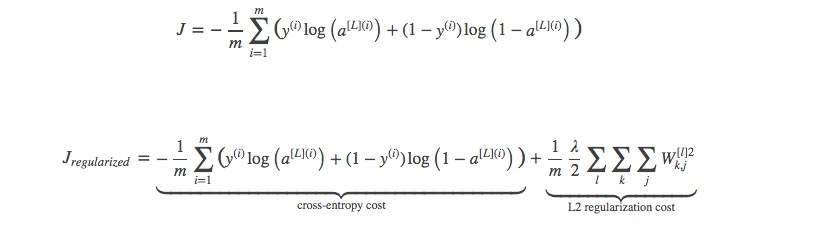
\includegraphics[width=5cm]  {19.jpg}}
 \caption{加一}
 \label{fig:19}
\end{figure}

矩阵的转置,A',转置两次(A')',又重新得到A矩阵。

还有一些有用的函数,比如:a=[1 15 2 0.5],这是一个1行4列矩阵,val=max(a),这将返回A矩阵中的最大值15。
[val, ind]=max(a),这将返回a矩阵中的最大值存入val,以及该值对应的索引,元素15对应的索引值为2存入ind,
所以ind等于2。如图~\ref{fig:20}所示。注意用命令max(A),A是一个矩阵的话,这样做就是对每一列求最大值。
\begin{figure}[H]
 \center{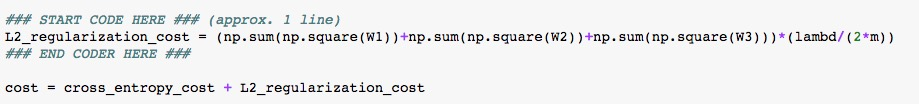
\includegraphics[width=6cm]  {20.jpg}}
 \caption{求最大值}
 \label{fig:20}
\end{figure}

输入 $a<3$,这将进行逐元素的运算,所有元素小于3的返回1,否则返回0。如果输入find(a$<$3),
输出小于3的元素的索引(下标从1开始)。如图~\ref{fig:21}所示。
\begin{figure}[H]
 \center{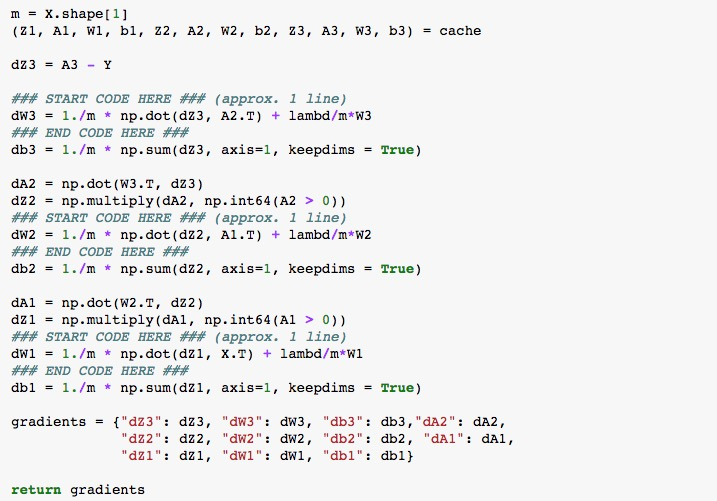
\includegraphics[width=6cm]  {21.jpg}}
 \caption{比较值}
 \label{fig:21}
\end{figure}

设A=magic(3),magic函数将返回一个矩阵,称为魔方阵或幻方(magic squares),数学性质:他们所有的行和列
和对角线加起来都等于相同的值。这在机器学习基本用不上,但是可以用这个方法很方便地生成一个3行3列的矩阵。

输入[r,c]=find(A>=7),这将找出A中大于等于7的所有元素的索引,因此,r和c分别表示行和列。如图~\ref{fig:22}所示。
\begin{figure}[H]
 \center{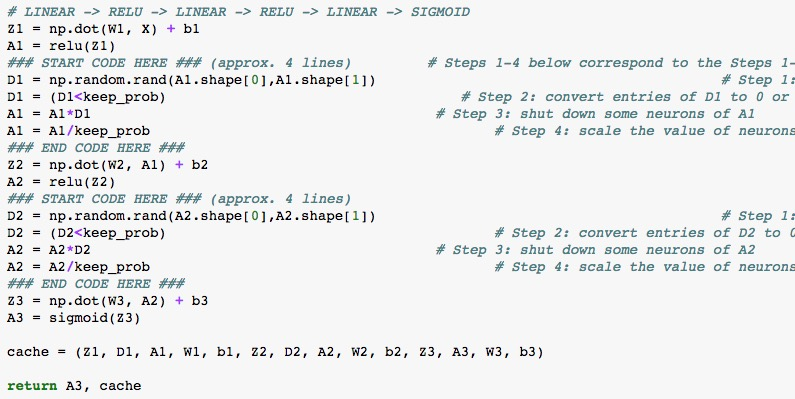
\includegraphics[width=5cm]  {22.jpg}}
 \caption{比较值}
 \label{fig:22}
\end{figure}

求和函数。sum(a),就是把a中的所有元素加起来了。乘积函数。键入 prod(a),
prod意思是乘积,它将返回这四个元素的乘积。四舍五入函数。floor(a)向下四舍五入,所以a中的0.5将被下舍变成0。
ceil(a),表示向上四舍五入,所以0.5将上舍入变为1。如图~\ref{fig:23}所示。
\begin{figure}[H]
 \center{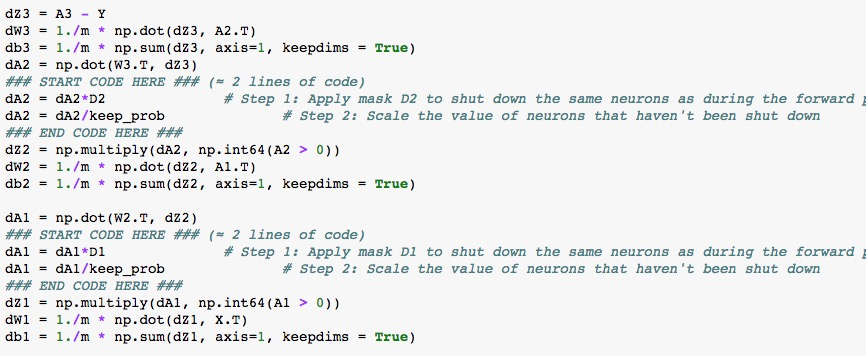
\includegraphics[width=6cm]  {23.jpg}}
 \caption{其它函数}
 \label{fig:23}
\end{figure}

键入type(3)(MATLAB中不是此用法),得到一个$3\times3$的矩阵,键入max[rand(3),rand(3)],这样做的结果是
返回两个$3\times3$的随机矩阵,并且逐元素比较取最大值。输入max(A,[],1),得到每一列的最大值,1表示取A矩阵第一个维度的
最大值。相对地,如果键入max(A,[],2),这将得到每一行的最大值。如图~\ref{fig:24}所示。
\begin{figure}[H]
 \center{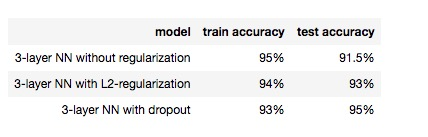
\includegraphics[width=6cm]  {24.jpg}}
 \caption{最大值}
 \label{fig:24}
\end{figure}

所以可以用这个方法求每一行或每一列的最值,另外,在默认情况下max(A)返回的是每一列的最大值,如果要找出
整个矩阵A的最大值,可以输入max(max(A)),或者将A矩阵转换为一个列向量,然后键入 max(A(:))。

 最后,A为9行9列的魔方阵,输入sum(A,1),得到每一列的和。sum(A,2),得到每一行的和。
 算对角线元素的和。首先构造一个$9\times9$的单位阵,键入 eye(9) ,然后用A逐点乘以这个单位矩阵,
 除了对角线元素外,其他元素都会得到0。键入sum(sum(A.$*$eye(9)))。如图~\ref{fig:25}所示。
 \begin{figure}[H]
  \center{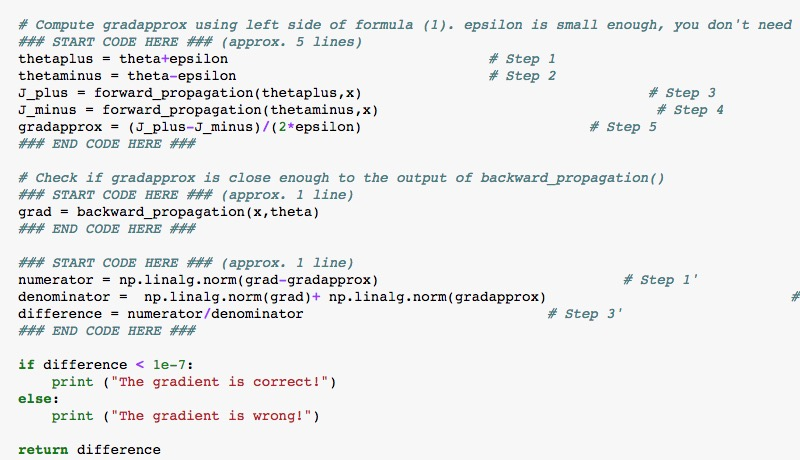
\includegraphics[width=8cm]  {25.jpg}}
  \caption{魔方矩阵求和}
  \label{fig:25}
 \end{figure}

flipup/flipud 表示向上/向下翻转。(matlab无此功能)
求逆矩阵,pinv(A)称为为逆矩阵,你就把它看成是矩阵A求逆,因此这就是A矩阵的逆矩阵。
设temp=pinv(A),然后再用temp乘以A,实际上得到的就是单位矩阵,对角线为1,其他元素为0。如图~\ref{fig:26}所示。
\begin{figure}[H]
 \center{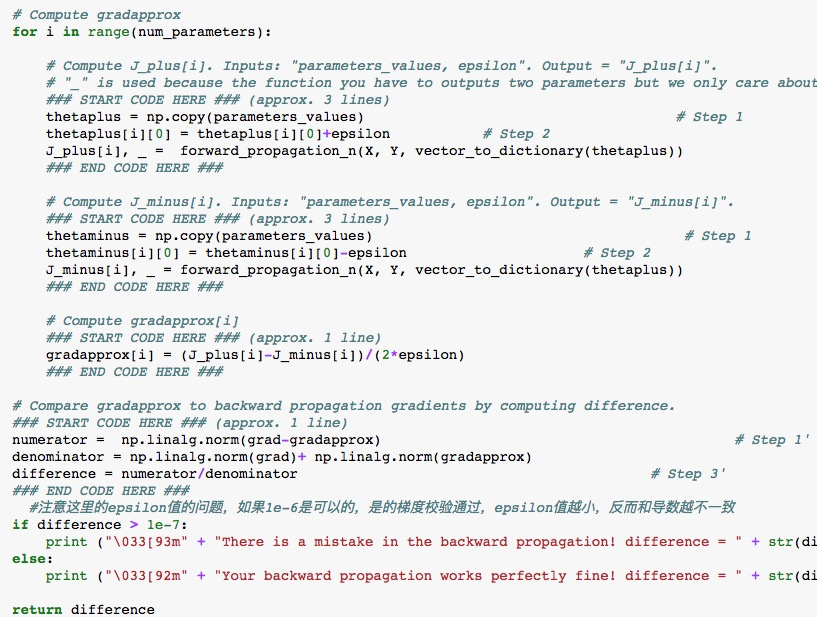
\includegraphics[width=6cm]  {26.jpg}}
 \caption{求逆}
 \label{fig:26}
\end{figure}

\subsection{Plotting Data 绘图数据}
之前的视频中,谈到绘制成本函数J($\theta$),可以帮助确认梯度下降算法是否收敛。
通常情况下,绘制数据或学习算法所有输出,会帮助改进学习算法。

首先快速生成一些数据用来绘图。

>> t=[0:0.01:0.98];
>> t
>> y1 = sin(2*pi*4*t);
>> plot(t,y1)

回车后得到图像。如图~\ref{fig:27}所示。
\begin{figure}[H]
 \center{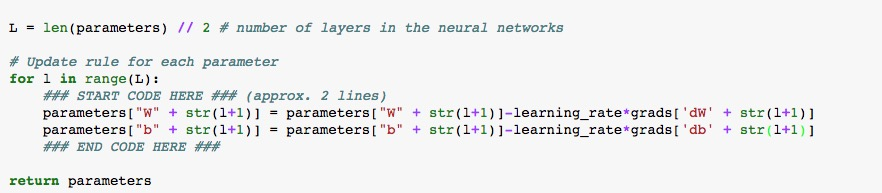
\includegraphics[width=6cm]  {27.jpg}}
 \caption{绘制sin图像}
 \label{fig:27}
\end{figure}
横轴是变量t,纵轴是y1,也就是我们刚刚所输出的正弦函数。

设置y2:

>> y2 = cos(2*pi*4*t);

>> plot(t,y2)

同时表示正弦和余弦曲线。

>> plot(t,y1)

>> hold on

>> plot(t,y2)

>> plot(t,y2,`r')

>> xlabel(`time')

>> ylabel(`value')

>> legend(`sin','cos')

>> title(`myplot')

输入:plot(t,y1),得到正弦函数,我使用函数hold on,hold on函数的功能是将新的图像绘制在旧的之上。
再绘制y2,输入:plot(t,y2)。要以不同的颜色绘制余弦函数,r代表所使用的颜色。xlabel(`time'),来标记X轴即水平轴,
ylabel(`value'),来标记垂直轴的值。legend(`sin',`cos')标记两条函数曲线。最后输入 title(`myplot'),在图像的顶部显示这幅图的标题。
如图~\ref{fig:28}所示。
\begin{figure}[H]
 \center{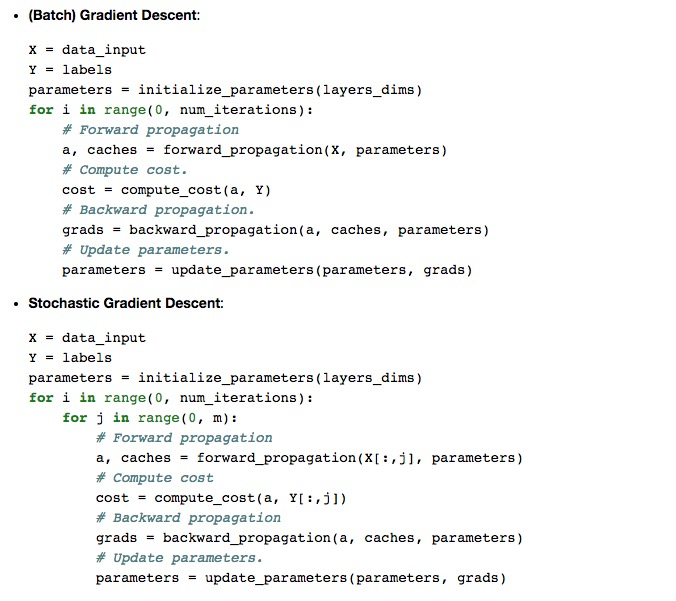
\includegraphics[width=6cm]  {28.jpg}}
 \caption{绘制sin、cos图像}
 \label{fig:28}
\end{figure}

如果你想保存这幅图像,你输入cd `地址' print -dpng`myplot.png',png是一个图像文件格式。

删掉图像close命令。Octave可以让你为图像标号。你键入figure;plot(t,y1);将显示第一张图,绘制了变量t y1。
键入figure(2);plot(t,y2);将显示第一张图,绘制了变量t y2。subplot命令。subplot(1,2,1),将图像分为一个
1$*$2的格子,就是前两个参数,然后它使用第一个格子:plot(t y1),也就是最后一个参数1的意思。如图~\ref{fig:29}所示。
\begin{figure}[H]
 \center{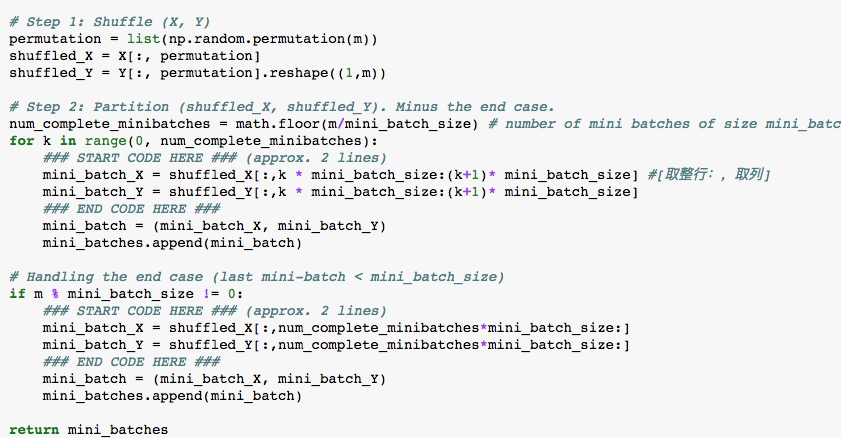
\includegraphics[width=6cm]  {29.jpg}}
 \caption{绘制sin、cos图像}
 \label{fig:29}
\end{figure}

最后一个命令,你可以改变轴的刻度,比如改成[0.5 1 -1 1],输入命令:axis([0.5 1 -1 1]),就是设置了右边图的x轴
和y轴的范围。

Clf(清除一幅图像)。

可视化矩阵,imagesc(A)命令,他将绘制一个$5*5$的矩阵,一个$5*5$的彩色格图,不同颜色对应矩阵中的不同值。
使用colorbar,命令imagesc(A),colorbar,colormap gray; 。实际上是在同一时间运行三个命令:运行imagesc,
然后运行colorbar,然后运行colormap grap。生成了一个颜色图像,一个灰度分布图,并在右边也加入一个颜色条。所以这个颜色条显示不同深浅的颜色所对应
的值。如图~\ref{fig:30}所示。
\begin{figure}[H]
 \center{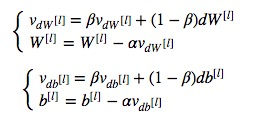
\includegraphics[width=6cm]  {30.jpg}}
 \caption{绘制矩阵}
 \label{fig:30}
\end{figure}

不同的方格对应于一个不同的灰度。输入 imagesc(magic(15)),colorbar,color gray。这将会是一副$15*15$的magic方阵值的图。
如图~\ref{fig:31}所示。
\begin{figure}[H]
 \center{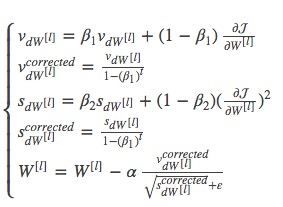
\includegraphics[width=6cm]  {31.jpg}}
 \caption{绘制矩阵}
 \label{fig:31}
\end{figure}

总结,上几条命令是用逗号进行连接函数调用。如果我键入a=1,b=2,c=3 然后一直按Enter键,其实这是将这三个命令同时执行,或者是将
三个命令一个接一个执行,他将输出所有这三个结果。Octave中分号连接不输出任何值,MATLAB分号返回最后一个表达式。

\subsection{For,while,if statements,and functions 控制语句:for,while,if语句}
控制语句的定义和使用。

首先,将V值设为一个10行1列的零向量:v=zeros(10,1)。接着用for循环,让i等于1到10,写出来就是i=1:10。设置V(i)的值等于2的i次方,循环最后写上
``end''。如图~\ref{fig:32}所示。
\begin{figure}[H]
 \center{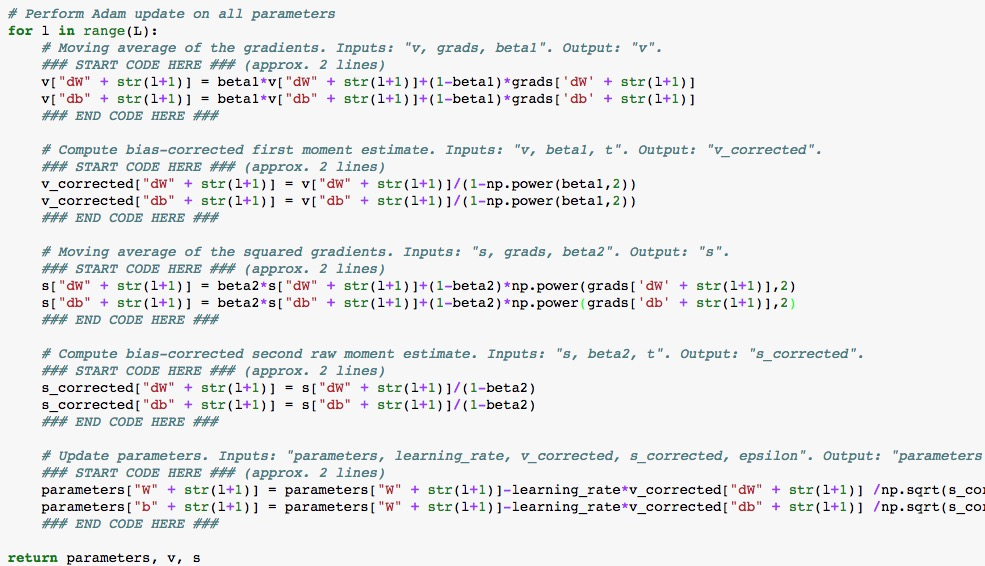
\includegraphics[width=6cm]  {32.jpg}}
 \caption{for循环}
 \label{fig:32}
\end{figure}

通过索引(indices)等于1到10: indices=1:10 ,这时indices就是一个从1到10的序列。i=indices,等价于直接把i写到1到10。
这时indices就是一个从1到10的序列。如图~\ref{fig:33}所示。
\begin{figure}[H]
 \center{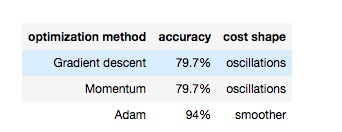
\includegraphics[width=4cm]  {33.jpg}}
 \caption{for循环}
 \label{fig:33}
\end{figure}

Octave里也有``break''和``continue''语句,你也可以在Octave环境李世勇 那些循环语句。

while循环语句。例子如图~\ref{fig:34}所示。
\begin{figure}[H]
 \center{\includegraphics[width=5cm]  {34.jpg}}
 \caption{whlie循环}
 \label{fig:34}
\end{figure}

if\-else语句。例子如图~\ref{fig:35}所示。
\begin{figure}[H]
 \center{\includegraphics[width=8cm]  {35.jpg}}
 \caption{if\-else语句}
 \label{fig:35}
\end{figure}

如果需要退出Octave,可以键入exit命令,然后回车就会退出,或者quit也可以。

如何定义和调用函数。

在桌面上存一个预先定义的文件名为``SquareThisnNmber.m''(文件名一定要和函数名一致),是在Octave环境下定义的函数。
用写字板程序来打开文件。如何在Octave里定义函数,文件只有三行。

function y = SquareThisNumber(x)

y = x\^{}2;

第一行意思是,告诉Octave,我想返回一个值,并且返回值被存放在变量y里。另外,告诉
Octave这个函数有一个参数x,还有定义的函数体,也就是y等于x的平方。尝试直接调用这个函数
SquareThisNumber(5),这是无法完成的。,Octave说这个方程为被定义。这是因为Octave不知道
不知道文件的路径。使用pwd查看路径,用cd将路径设为文件所在位置。再次调用函数,可以运行。
如图~\ref{fig:36}所示。
\begin{figure}[H]
 \center{\includegraphics[width=8cm]  {36.jpg}}
 \caption{定义调用函数}
 \label{fig:36}
\end{figure}

一个更高级的功能,``search path(搜索路径)'',使用addpath命令添加路径,添加路径将该目录添加到Octave的搜索路径,
这样即使跑到其他路径下,Octave依然知道会在文件所在路径下寻找函数。如图~\ref{fig:37}所示。
如图~\ref{fig:37}所示。
\begin{figure}[H]
 \center{\includegraphics[width=8cm]  {37.jpg}}
 \caption{添加路径}
 \label{fig:37}
\end{figure}

Octave还有一个其他许多编程语言都没有的概念,就是可以允许定义一个函数,使得返回值是多个值或多个参数。
例子,定义一个函数``SquareAndCubeThisNumber(x)''(x的平方以及x的立方)。返回值时两个y1 y2。

function [y1,y2]$=$SquareAndCubeThisNumber(x)

$y1=x^2$;

$y2=x^3$;

如果键入[a,b]$=$SquareAndCubeThisNumber(5),然后,a$=$25 b$=$125。

复杂例子。有一个数据集,数据点为[1,1],[2,2],[3,3]。用Octave函数来计算代价函数$J(\theta)$,
就是计算不同的$\theta$所对应的代价函数值J。

首先把数据放到Octave里,X=[1 1;1 2;1 3];如图~\ref{fig:38}所示。
\begin{figure}[H]
 \center{\includegraphics[width=7cm]  {38.jpg}}
 \caption{数据}
 \label{fig:38}
\end{figure}

写一个函数costFunctionJ.m。如图~\ref{fig:39}所示。
\begin{figure}[H]
 \center{\includegraphics[width=8cm]  {39.jpg}}
 \caption{计算代价函数}
 \label{fig:39}
\end{figure}

在Octave里运行。如图~\ref{fig:40}所示。
\begin{figure}[H]
 \center{\includegraphics[width=7cm]  {40.jpg}}
 \caption{计算代价函数}
 \label{fig:40}
\end{figure}

设置 $\theta$0 等于 0,$\theta$1 等于 1,恰好 45 度的斜线,这条线是可以完美拟合数据集的。
而相反地,如果设置 theta 等于[0; 0],那么这个假设就是 0 是所有的预测值,和刚才 一样,
设置 $\theta$0 = 0,$\theta$1 也等于 0,然后我计算的代价函数,结果是 2.333。
实际就等于1 的平方,也就是第一个样本的平方误差,加上 2 的平方,加上 3 的平方,然后除以 2m,
也就是训练样本数的两倍,这就是 2.33。如图~\ref{fig:41}所示。
\begin{figure}[H]
 \center{\includegraphics[width=7cm]  {41.jpg}}
 \caption{计算代价函数}
 \label{fig:41}
\end{figure}

确实是可以计算出正确的代价函数的。至少基于这里的 X 和 y 是成立的。也就是我们这几 个简单的训练集,至少是成立的。

\subsection{Vetorization 向量化}
无论你是用 Octave,还是别的语言,比如 MATLAB 或者你正在用 Python、NumPy 或 Java C C++,所有这些语言都具有各种线性代数库,
这些库文件都是内置的,容易阅读和获取,他们通常写得很好,已经经过高度优化,通常是数值计算方面的博士或者专业人士开发的。
优点:首先,这样更有效,也就是说运行速度更快,并且更好地利用你的计算机里可能有 的一些并行硬件系统等等(first, is more efficient,
so you just run more quickly and take better advantage of any parallel hardware your computer may have and so on. );其次,
这也意味着你可以用更少的代码来实现你需要的功能(it also means that you end up with less code that you need to write,
so it's a simpler implementation that is therefore maybe also more likely to be by free.)。因此,实现的方式更简单,代码出现问题的有可能性也就越小。

Vectorization example.这是一个常见的线性回归假设函数:
\begin{equation*}
h_{\theta } \left ( x \right )= \sum_{j= 0}^{n}\theta _{j}x_{j}
\end{equation*}

如果要计算$h_{\theta}(x)$,把它看作$\theta^{T}x$,可以写成两个向量的内积:
\begin{equation*}
  \theta=
  \begin{bmatrix}
     \theta_{0} \\
     \theta_{1} \\
     \theta_{2} \\
  \end{bmatrix}
  x=
\begin{bmatrix}
  x_{0} \\
   x_{1} \\
   x_{2} \\
\end{bmatrix}
\end{equation*}

Unvectorized implementation(变形):

prediction = 0.0;

for j= 1:n+1,

    prediction = prediction + theta(j) * x(j)

end;

计算$h_{\theta}(x)$是未向量化的。注意:这里的向量用下标是0,但因为MATLB的下标
从1开始,在MATLAB中$\theta_{0}$可能用$\theta_{1}$来表示,从1开始。
\newline

Vectorized implementation:

prediction = theta' * x;

把$\theta$和x看做向量,只需要令变量 prediction 等于 theta 转置乘以 x。
这行代码就是利用 Octave 的高度优化的数值,线性代数算法来计算两个向量$\theta$以及 x 的内积,
这样向量化的 实现更简单,它运行起来也将更加高效。

这就是 Octave 所做的而向量化的方法,在其他编程语言中同样可以实现。让我们来看 一个 C++ 的例子,
如图~\ref{fig:42}所示。
\begin{figure}[H]
 \center{\includegraphics[width=10cm]  {42.jpg}}
 \caption{向量化vs非向量化}
 \label{fig:42}
\end{figure}

使用较好的 C++ 数值线性代数库library ,你可以写出像右边这样的代码。

一个更为复杂的例子,这是线性回归算法梯度下降(gradient descent of a linear ragression)的更新规则:
\begin{equation*}
  \theta_0 := \theta_0 - \alpha
  \frac{1}{m}
  \sum^m_{\substack{i=1}}
   \Big(h_\theta(x^{(i)})-y^{(i)}\Big)x_{0}^{(i)}
\end{equation*}
\begin{equation*}
   \theta_1 := \theta_1 - \alpha
   \frac{1}{m}
   \sum^m_{\substack{i=1}}
    \Big(h_\theta(x^{(i)})-y^{(i)}\Big)x_{1}^{(i)}
\end{equation*}
\begin{equation*}
  \theta_2 := \theta_2 - \alpha
  \frac{1}{m}
  \sum^m_{\substack{i=1}}
   \Big(h_\theta(x^{(i)})-y^{(i)}\Big)x_{2}^{(i)}
\end{equation*}

n=2

可以想象实现这三个方程的方式之一,就是用一个 for 循环,就是让 j 等于 0、等于 1、等于 2,来更新 $\theta_{j}$。

用向量化的方式来实现,把 $\theta$ 看做一个向量,然后我用 $\theta-\alpha$ 乘以某个别的向量$\delta$ 来更新$\theta$ 。

$\delta$ 等于:
\begin{equation*}
\delta=
\frac{1}{m}
\sum^m_{\substack{i=1}}
 \Big(h_\theta(x^{(i)})-y^{(i)}\Big)x^{(i)}
\end{equation*}

把 $\theta$看作一个向量,有一个 n+1 维向量,$\alpha$ 是一个实数,$\delta$ 在这里是一个向量。
如图~\ref{fig:43}所示。
\begin{figure}[H]
 \center{\includegraphics[width=10cm]  {43.jpg}}
 \caption{等价式子}
 \label{fig:43}
\end{figure}

Vectorized implementation:
\begin{equation*}
\theta : = \theta - \alpha \delta
\end{equation*}

那么什么是向量$\delta$,和 $x^{i}$?
\begin{equation*}
  \delta=
  \begin{bmatrix}
     \delta_{0} \\
     \delta_{1} \\
     \delta_{2} \\
  \end{bmatrix}
  x^{(i)}
\begin{bmatrix}
  x_{0}^{(i)} \\
   x_{1}^{(i)} \\
   x_{2}^{(i)} \\
\end{bmatrix}
\end{equation*}

有时我们使用几十或几百个特征量来计算线性归回,当你使用向量化地实现线性回归,
通常运行速度就会比你以前用你的 for 循环快的多。




\end{document}
